\documentclass{article}
\usepackage[utf8]{inputenc}
\usepackage[margin = 0.8in]{geometry}
\usepackage{graphicx}
\usepackage{amsmath, amssymb}
\usepackage{subcaption}
\usepackage{multirow}
\usepackage{mathtools}
\usepackage{float}


\title{RBE595 - Week 6 Assignment}
\author{Keith Chester}
\date{Due date: February 19, 2023}

\begin{document}
\maketitle

In this assignment, we looked at a simple stochastic environment of 6 consecutive cells, labeled 0 through 4. Either end of the line of cells were terminal states - cell 0 with a reward of 1, cell 5 with a reward of 5. All other cells were a reward of 0 with a choice to go either left or right. There existed an 80\% chance of the robot in our environment following the designated action, a 15\% chance of the robot merely staying where it is, and a 5\% chance for the robot to go the opposite of what was chosen.

Here we developed two Monte Carlo agents - an exploring starts agent and a first visit agent. We looked at the convergence of the agent at the end of a set number of episodes, from 1 episode to 500 episodes. For each of these episodes, we performed the test with 100 different agents. We then looked at the average $Q(s,a)$ of each state/action pair, as well as the $V(s)$ of each.

\begin{figure}
    \centering
    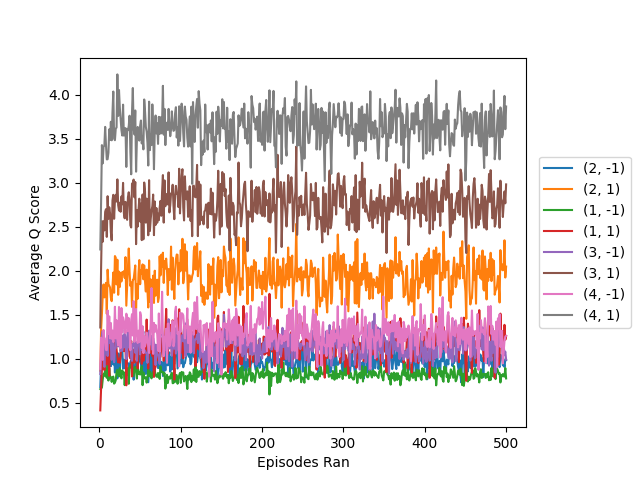
\includegraphics[width = 0.8\textwidth]{results_exploring_start_q.png}
    \caption{Q(s,a) Avg for Exploring Starts Monte Carlo Agent}
\end{figure}

\begin{figure}
    \centering
    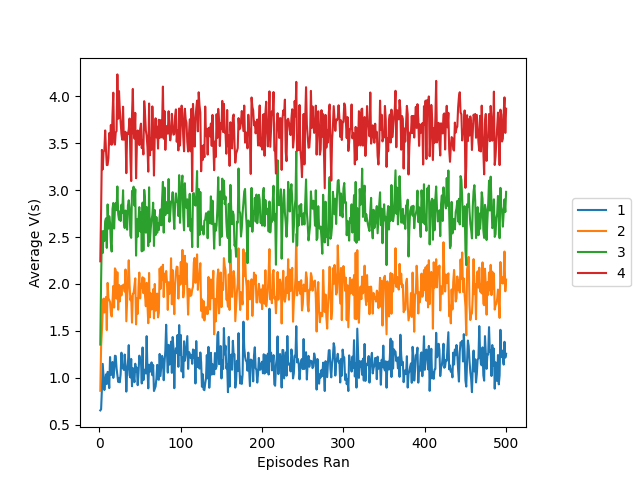
\includegraphics[width = 0.8\textwidth]{results_exploring_start_v.png}
    \caption{V(s) Avg for Exploring Starts Monte Carlo Agent}
\end{figure}

\begin{figure}
    \centering
    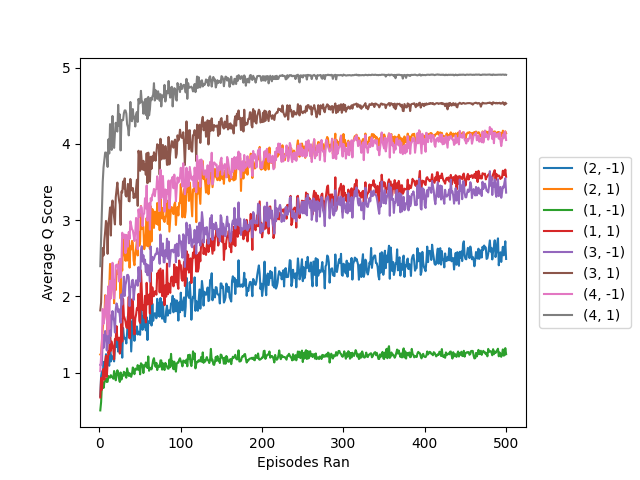
\includegraphics[width = 0.8\textwidth]{results_first_visit_q.png}
    \caption{Q(s,a) Avg for First Visit Monte Carlo Agent}
\end{figure}

\begin{figure}
    \centering
    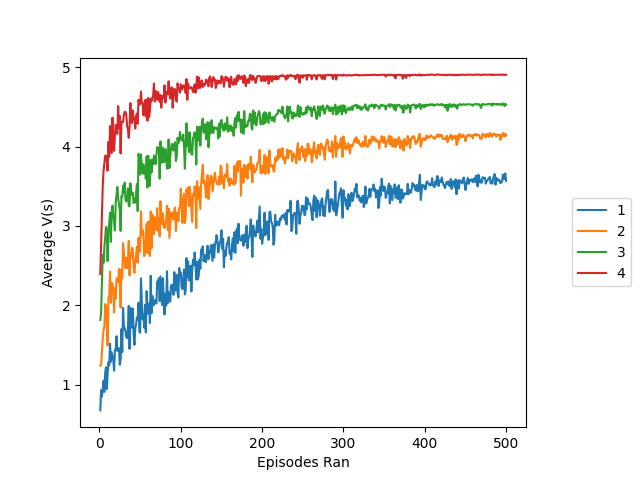
\includegraphics[width = 0.8\textwidth]{results_first_visit_v.png}
    \caption{V(s) Avg for First Visit Monte Carlo Agent}
\end{figure}

Our convergence for exploring starts is chaotic as it sometimes "locks in" an incorrect approach; this is likely due to our enviroment. Exploring starts gets it exploration via random starts, but because of our small environment it quickly learns its policy and sticks to it. This means that, if in our initialization of all values we have relatively equal values for everything and thus true randomness at the start, we can learn and lock in a policy for exploring starts that is the exact opposite of true optimal. This can occur at first in first-visit, but because of the $\epsilon$-greedy approach for exploration this will be corrected over a long enough run of episodes. I suspect that, had we a larger or more complex environment, exploring starts would have had a better showing on convergence towards the expected optimal policy. Note that it is because of this variance of start for exploring start that led me to run 100 attempts per set of episodes to try and find a smoothed expectation from the agents.



\end{document}
